\section[User Interface Design]{\hyperlink{toc}{User Interface Design}}
	\label{sec:userInterfaceDesign}
	
	This section describes precisely the mockups already presented in the \emph{SafeStreets: Requirements Analytics and Specification Document} \cite{RASD} in order to understand how the main functionalities will be offered. The first subsection focuses on the illustration of the flow of both the mobile and the web applications designed for the users and the authorities by using two \textbf{UX diagrams}.\\
	
	As the design of the application defines two different interfaces, one for the users and one for the authorities, the following subsections will present each the related interfaces. These mockups are meant to precisely define how the customers will interact with the system to benefit of its functionalities, their design is still minimal not to reduce too much the style and fantasy of the developers. In fact it has to be considered that the \textbf{Mobile Application} for the users will possibly have two different styles related to the \emph{Android} and \emph{Apple} layouts while the \textbf{Web Application} can be designed with any kind of technology preferred.\\
	
	Both the interactions are structured over a \emph{Client-Server} paradigm, hence all the actions performed by a client are managed by the respective logic that allows to display the graphical interface and whenever a request is needed, its execution will be deployed to the server. Once the answer is received back, the modules for the presentation will display its information to the customers.
	
	\subsection[UX Diagrams]{\hyperlink{toc}{UX Diagrams}}
		\label{sec:uxDiagrams}
		
		Before going deep in details that describe the interfaces of the applications designed for both the users and the authorities, it is very useful to first understand how these interfaces interact one with the others by means of a flow graph that leads from one mockup to the other. Thanks to this kind of diagrams, called UX diagrams, we are now able to understand in which way either the user or the authority will have to interact with the application in order to benefit of the services provided by SafeStreets.
		
		\newpage
		
		\subsubsection[User Mobile Application]{\hyperlink{toc}{User Mobile Application}}
			\label{sec:userUXDiagram}
		
			\begin{figure}[ht!]
				\centering
				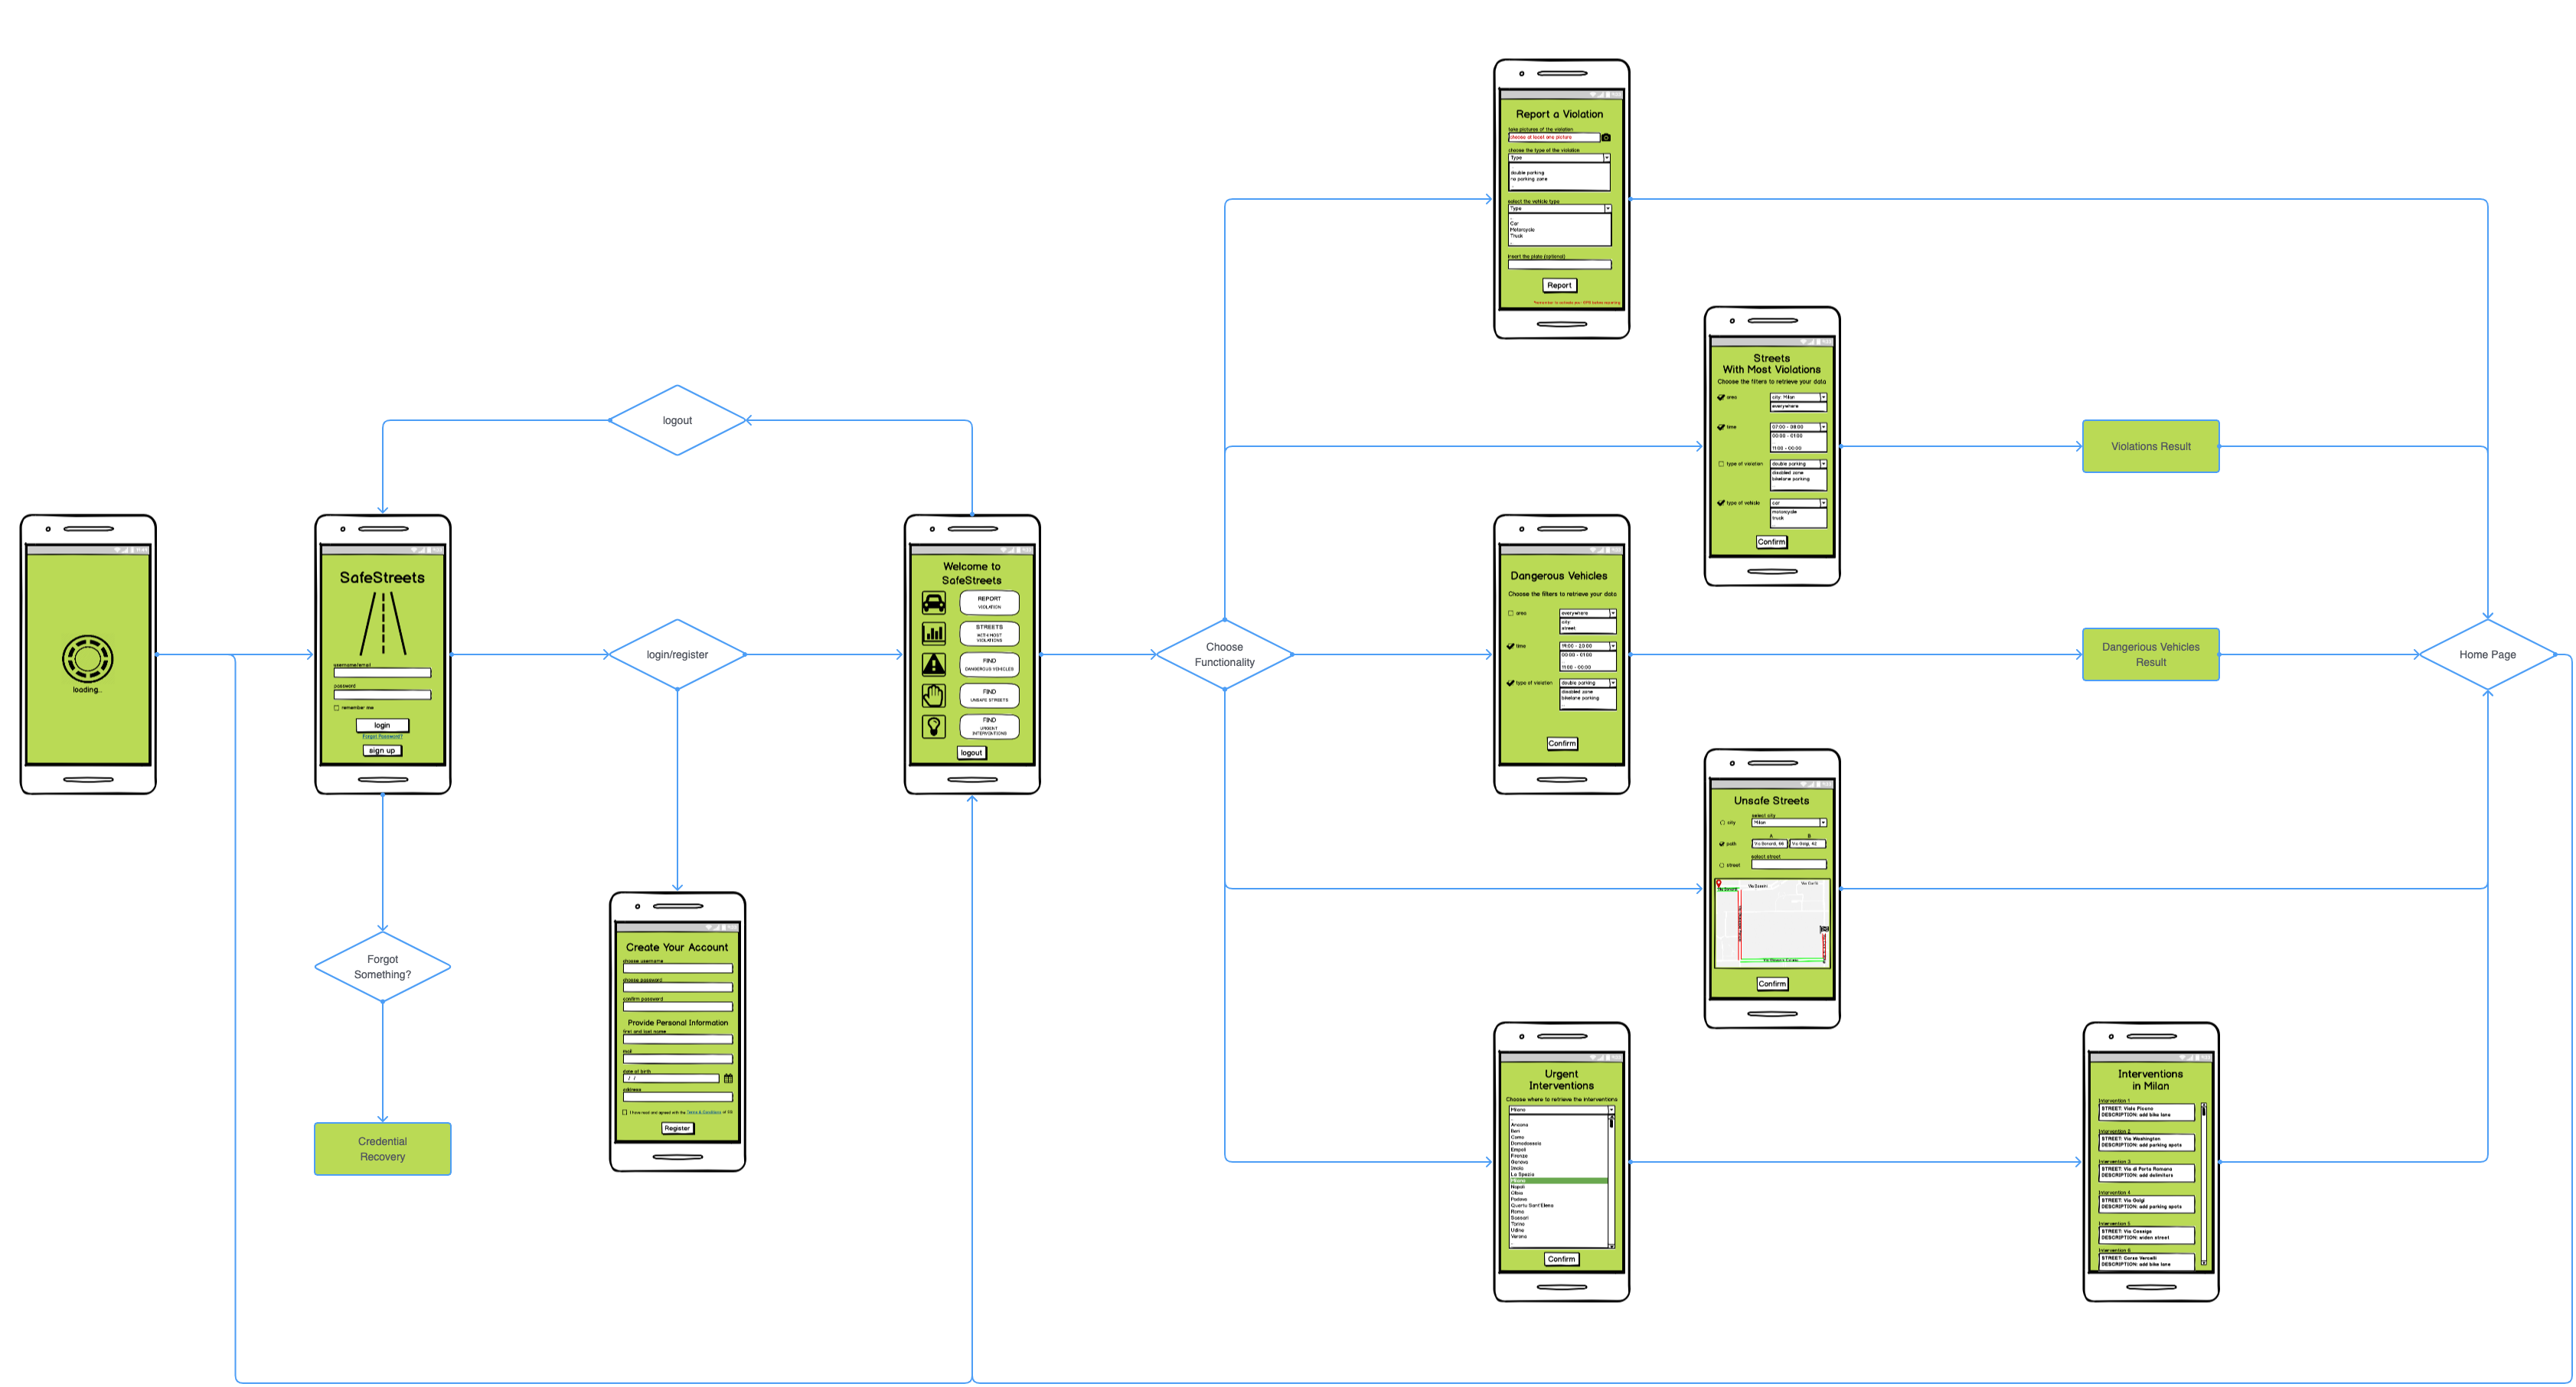
\includegraphics[scale=0.16, angle=90]{/diagrams/UX/userAppFlow.png}
				\caption{\label{fig:userAppFlow} Mobile Application UX Diagram}
			\end{figure}
		
			\FloatBarrier
		
		\subsubsection[Authority Web Application]{\hyperlink{toc}{Authority Web Application}}
			\label{sec:authorityUXDiagram}
			
			\begin{figure}[ht!]
				\centering
				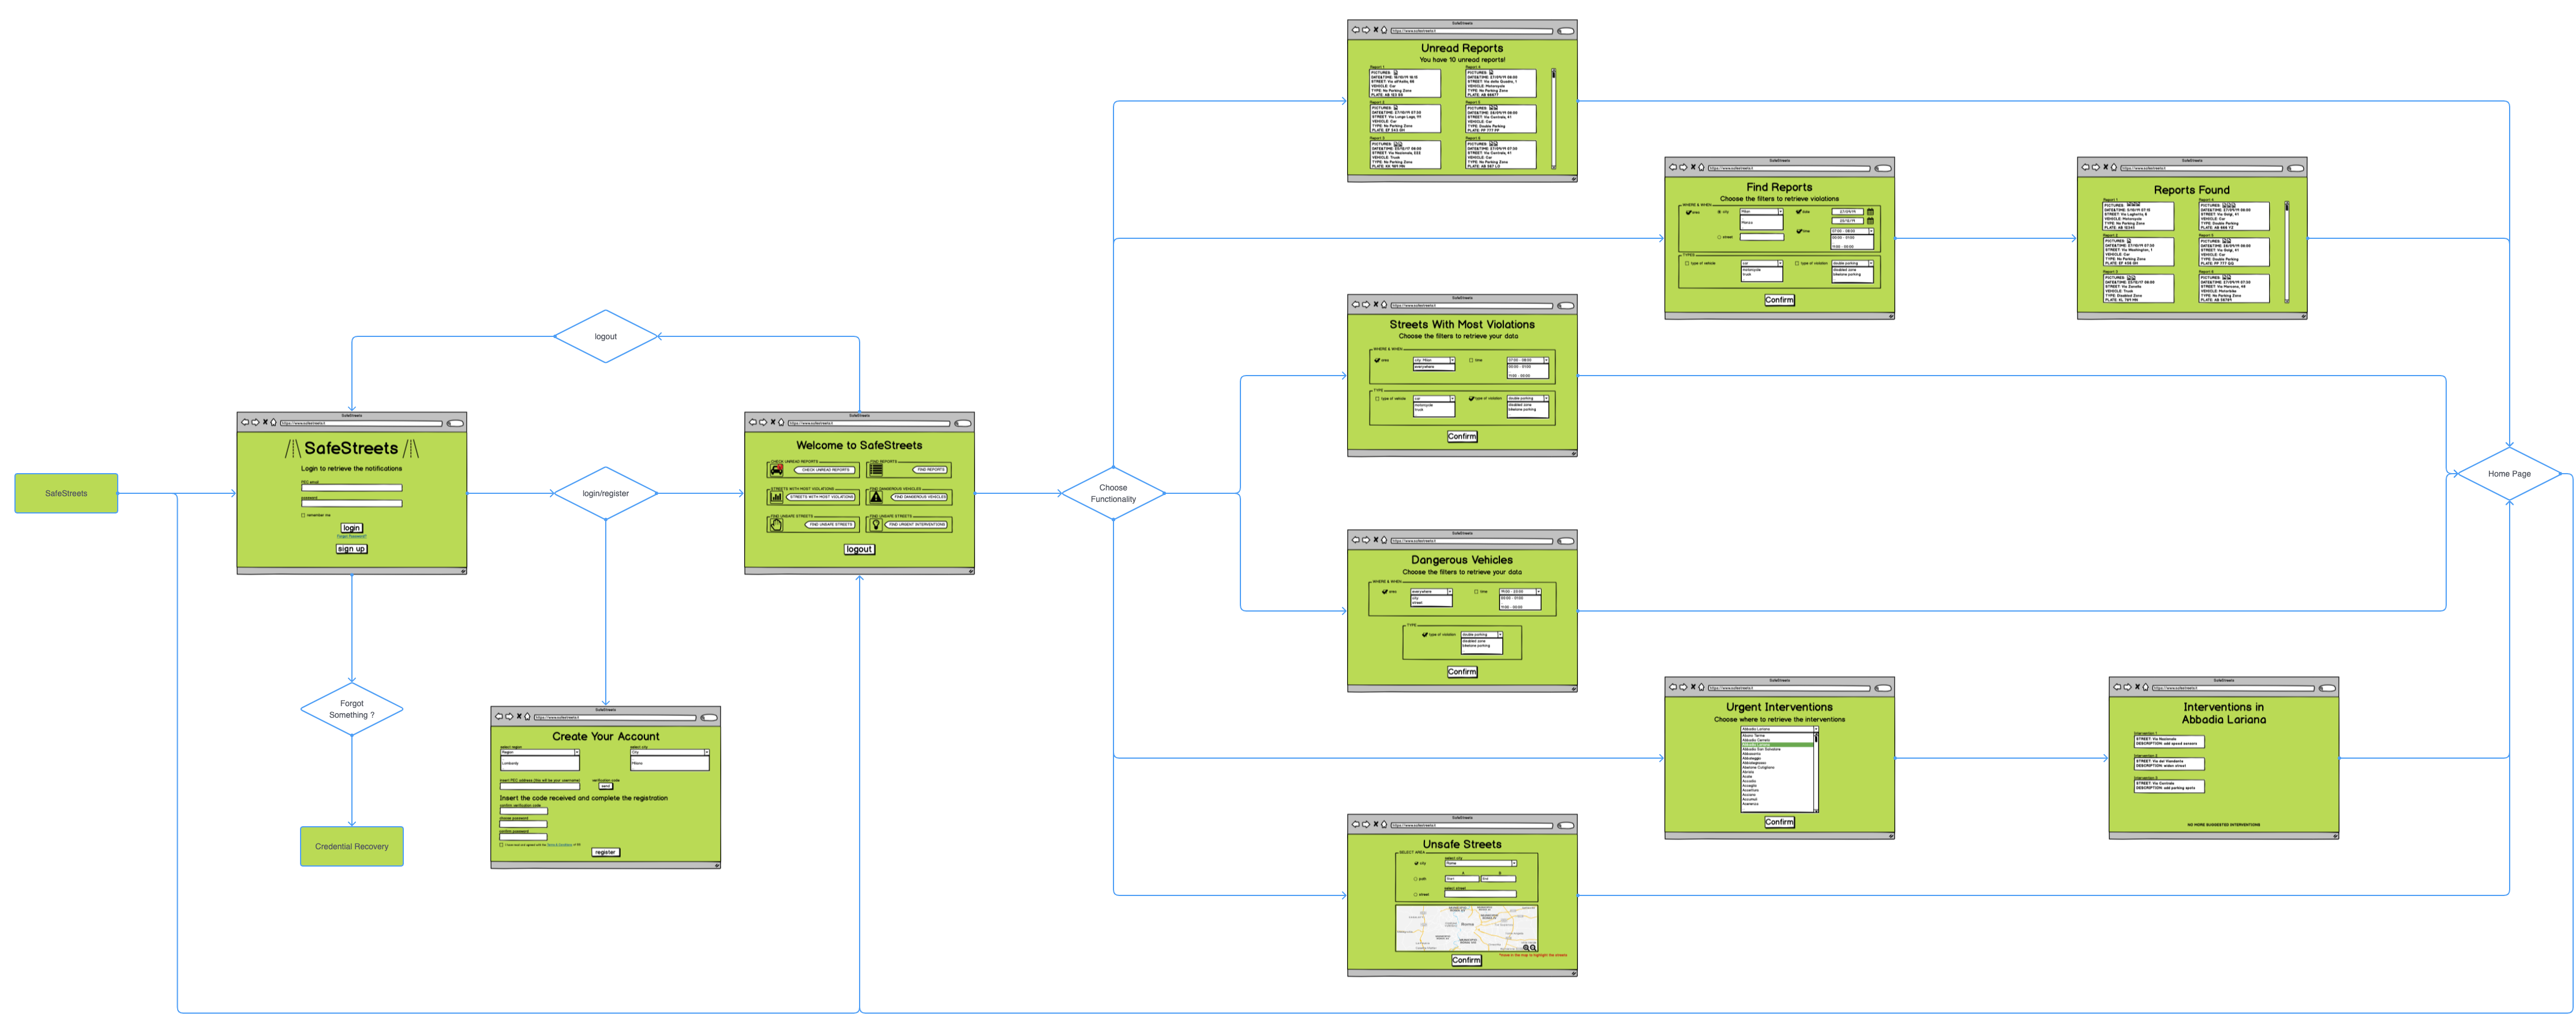
\includegraphics[scale=0.12, angle=90]{/diagrams/UX/authorityWebFlow.png}
				\caption{\label{fig:authorityAppFlow} Web Application UX Diagram}
			\end{figure}
		
			\FloatBarrier
			
	\subsection[User Mobile App]{\hyperlink{toc}{User Mobile App}}
		\label{sec:userMobileApp}
		
		As previously said the following mockups are just to define which functionalities each interface needs to present. Its layout is left unspecified to allow the creativity of the developer to consider also the two possible different layouts. However it is important to say that the \textbf{Mobile App} will be used by the users, citizens of any age, in possible uncomfortable moments. Hence it has to be intuitive and charming in particular to allow a quick way to report a notification. The interfaces that display the information relative to the mining functionalities has also to be easy to understand as it can be understood by any kind of user.
		
		\subsubsection[Login \& Registration]{\hyperlink{toc}{Login \& Registration}}
			\label{sec:userLoginRegistration}
			
			\paragraph{Login}
				The first mockup (\autoref{fig:loginApp}) is the initial page every user will find the first time he uses SafeStreets. A user can interact with the system only if authenticated. Hence the first time every user will choose the button \textbf{sign up} for registering to the system and interact with the page described in the next paragraph.\\
				
				If a user is already registered but has not chosen to be remembered, he will need to \textbf{login} to SafeStreet every time by providing either its username or email and his password. Once recognized he will be redirected to the home page of the application described in the next section.\\
				
				This interface leads also to the possibility of recovering the credentials in case a user forgets its password; the mockup relative to the link \textbf{Forgot Password?} in the application is not presented as it will simply ask for the users' email in order to send him his new password (the username recovery is not needed as the access can be always performed with the email).
				
			\paragraph{Registration}
				The registration (\autoref{fig:registrationApp}) allows the user to create his account in order to be authenticated whenever he chooses to use SafeStreets. Thanks to this interface he will be able to provide first the information related to his new account and then his personal details. At the end of the page, before confirming the registration it is mandatory that the user accepts the \textbf{Terms and Conditions} of SafeStreets.\\
				
				The button \textbf{register} will add the new user to the system and redirect to the login interface where the client can now access the system with the information provided in the previous module.
				
			\vspace{0.6cm}
				
			\begin{figure}[ht!]
				\centering
				\begin{minipage}{0.5\textwidth}
					\centering
					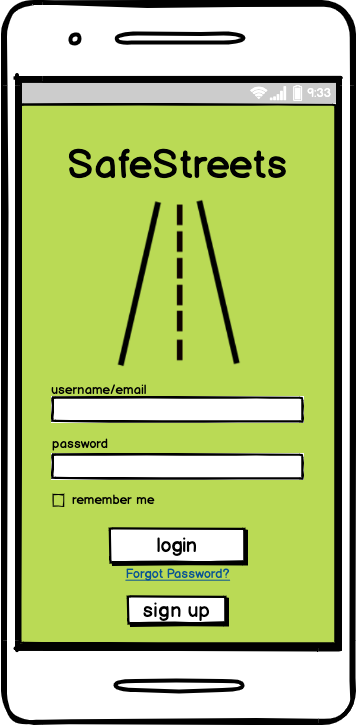
\includegraphics[width=0.8\textwidth]{/mockups/user/loginApp.png}
					\caption{\label{fig:loginApp} User Login}
				\end{minipage}\hfill
				\begin{minipage}{0.5\textwidth}
					\centering
					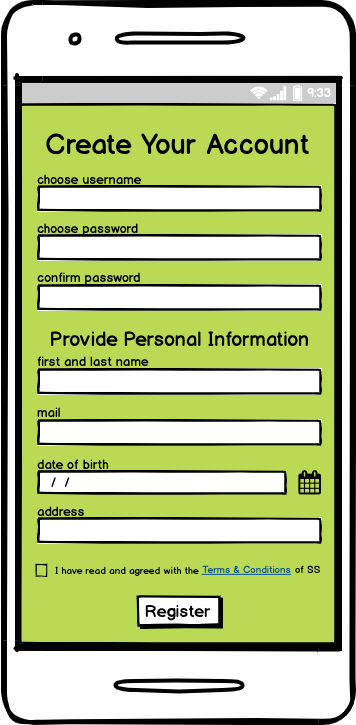
\includegraphics[width=0.8\textwidth]{/mockups/user/registrationApp.png}
					\caption{\label{fig:registrationApp} User Registration}
				\end{minipage}
			\end{figure}
		
			\FloatBarrier
		\subsubsection[Home Page]{\hyperlink{toc}{Home Page}}
			\label{sec:userHomePage}
			
			This page (\autoref{fig:homeApp}) is the core of the interfaces, once logged the user will reach it and after each action too. From the \textbf{Home Page} a user is able to perform all the functionalities allowed to him, offered by SafeStreets:
			
			\begin{itemize}
				\item Report Violation
				\item Streets With Most Violations
				\item Find Dangerous Vehicles
				\item Find Unsafe Streets
				\item Find Urgent Interventions
			\end{itemize}
		
			The \textbf{logout} button is used to log out of the application and thus the redirection will lead to the login page.\\
			
			\begin{figure}[ht!]
				\centering
				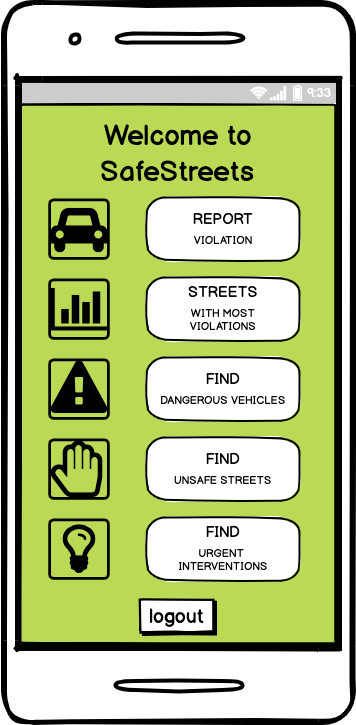
\includegraphics[scale=0.4]{/mockups/user/homeApp.png}
				\caption{\label{fig:homeApp} User Home}
			\end{figure}
		
			\FloatBarrier

		\subsubsection[Report Violation]{\hyperlink{toc}{Report Violation}}
			\label{sec:userReportViolation}
			
			This interface (\autoref{fig:notificationApp}) allows the entire process of notification to be held. It provides the user a way to insert all the possible information related to a parking violation in order to notify the authority. First the user is asked to take at least one picture of the violation and after to provide two other mandatory details: the type of the violation and the type of the vehicle he is reporting. In the end the plate's number can be also inserted, as we said this information is not mandatory because it is thought that the \emph{Image Recognition Algorithms} can determine it even without this help.\\
			
			It is important to remember that the device that is reporting the violation must have enabled its GPS to complete a notification. The position will be in fact added to the details of the notification once the user has pressed the \textbf{Report} button as the system can automatically retrieve the street where the infraction occurred.\\
			
			The entire data received whenever a user performs a report is the one that needs to be processed by the system before storing it. In fact it is necessary that no incorrect parking violation is taken into account by the system that wants to notify the authority whenever a new one is received.
			
			\begin{figure}[ht!]
				\centering
				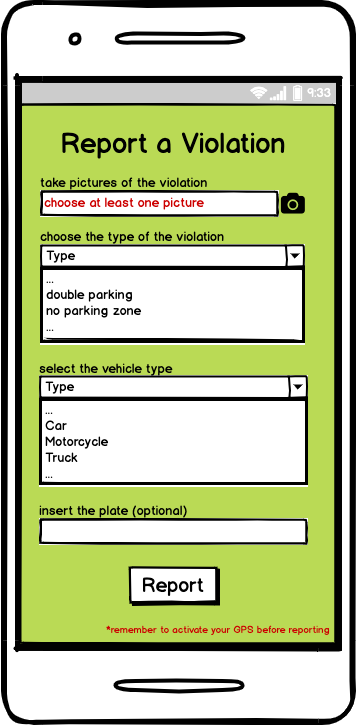
\includegraphics[scale=0.35]{/mockups/user/notificationApp.png}
				\caption{\label{fig:notificationApp} User Notification}
			\end{figure}
		
		\subsubsection[Basic Functionalities]{\hyperlink{toc}{Basic Functionalities}}
			\label{sec:userBasicFunctionalities}
			
			These mockups are the ones that allow the user to benefit of the basic functionalities, such as: mining the number of violations in a particular place or the vehicles that commit the most violations. Both the interfaces display the filters that a user can choose while mining the information, remember that the type of filters allowed for each functionality are different, depending on how the goals of the system have been specified.
			
			\paragraph{Streets With Most Violations}
			This page (\autoref{fig:violationsFrequencyApp}) is used to mine the information about the frequency of the violations that have already occurred. Data can be retrieved with different levels of aggregation thanks to the possible filters:
			
			\begin{itemize}
				\item \textbf{area:} by city or everywhere
				\item \textbf{time:} time slots of one hour each
				\item \textbf{type of violation:} different types of parking violations possible
				\item \textbf{type of vehicle:} different types of vehicle possible
			\end{itemize}
		
			Selected the filters and the parameters for each filter chosen, the user confirms the request with the \textbf{Confirm} button and receives the list of all the streets contained in the parking violations that match the parameters, ordered by the number of infractions.\\
			
			The mockup related to the result of this functionality is not presented because it simply has to display the list of the streets found and allow the user to get back to the home page.
			
			\paragraph{Dangerous Vehicles}
			This page (\autoref{fig:dangerousVechiclesApp}) is used to mine the information about the vehicles that commit the highest number of parking violations. As well as in the first functionality we have filters to retrieve the data, but only the ones that are interesting for this kind of request:
			
			\begin{itemize}
				\item \textbf{area:} by city, street or everywhere
				\item \textbf{time:} time slots of one hour each
				\item \textbf{type of violation:} different types of parking violations possible
			\end{itemize}
		
			Selected the filters and the parameters for each filter chosen, the user confirms the request with the \textbf{Confirm} button and receives the list of all the type of vehicles contained in the parking violations that match the parameters, ordered by the number of infractions.\\
			
			The mockup related to the result of this functionality is not presented because it simply has to display the list of the type of vehicles found and allow the user to get back to the home page.
			
			\vspace{0.6cm}
			
			\begin{figure}[ht!]
				\centering
				\begin{minipage}{0.5\textwidth}
					\centering
					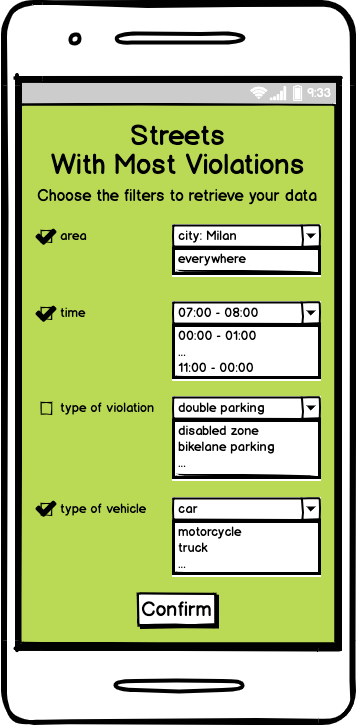
\includegraphics[width=0.7\textwidth]{/mockups/user/violationsFrequencyApp.png}
					\caption{\label{fig:violationsFrequencyApp} User Violations Frequency}
				\end{minipage}\hfill
				\begin{minipage}{0.5\textwidth}
					\centering
					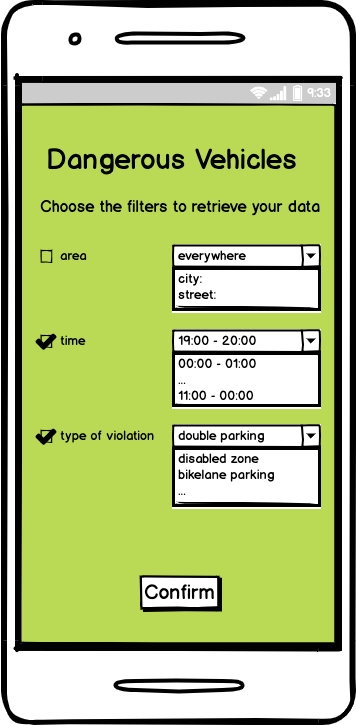
\includegraphics[width=0.7\textwidth]{/mockups/user/dangerousVehiclesApp.png}
					\caption{\label{fig:dangerousVechiclesApp} User Dangerous Vehicles}
				\end{minipage}
			\end{figure}
		
		\subsubsection[Advanced Functionalities]{\hyperlink{toc}{Advanced Functionalities}}
			\label{sec:userAdvancedFunctionalities}
			
			These mockups are the ones that allow the user to benefit of the advanced functionalities, such as: finding the safety of the streets and receive a suggestion for a possible intervention that can be considered in order to enhance the safety of a dangerous street. In this case we have multiple filters for the safety, related to the area the user decides to highlight while for the suggestions there is only one filter that selects the city of interest.
			
			\paragraph{Unsafe Streets}
			This page (\autoref{fig:unsafeStreetsApp}) is the only one that reflects the safety functionality, in fact whenever the user confirms the request with the \textbf{Confirm}
			button, the map on the bottom will be highlighted in green and red depending on the safety of the streets of interest. The selection of the area can be done in three different ways thanks to the filters provided by the interface:
			
			\begin{itemize}
				\item \textbf{city:} list of all the Italian cities
				\item \textbf{path:} two cells allow to select the starting (A) and the ending (B) point, the system will highlight the streets in the best path from A to B
				\item \textbf{street:} free choice of the user, a comma has to divide the street from the city
			\end{itemize}
		
			Once the user has chosen the area to highlight the safety and pressed the \textbf{Confirm} button, the map will be updated focusing on either the street or the path or the city, in this last case it will be displayed the view of the city with a high scale; in this last case a high view of the city will be displayed and the user will be able to zoom in and out to select the places it prefers.
			
			\begin{figure}[ht!]
				\centering
				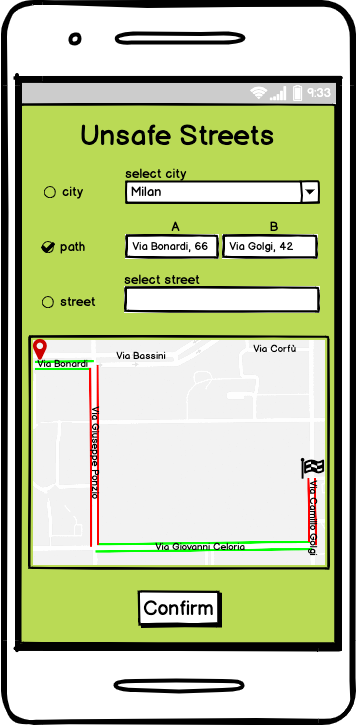
\includegraphics[scale=0.32]{/mockups/user/unsafeStreetsApp.png}
				\caption{\label{fig:unsafeStreetsApp} User Unsafe Streets}
			\end{figure}
		
			\paragraph{Urgent Interventions}
			This page (\autoref{fig:urgentInterventionsApp}) allows the user to retrieve the suggestions for the possible interventions in the city he selects. The \textbf{confirm} button will lead to the result providing a list of all the interventions found in that city.\\
			
			In this case we provide also the page of the results (\autoref{fig:interventionsFoundApp}) as it is important to show which kind of information this request will display. As we see in the result, for each intervention it is provided the street and the suggestion, in case a street has multiple suggestions, two interventions in the same street but with different suggestion will be presented.
			
			\vspace{0.6cm}
			
			\begin{figure}[ht!]
				\centering
				\begin{minipage}{0.5\textwidth}
					\centering
					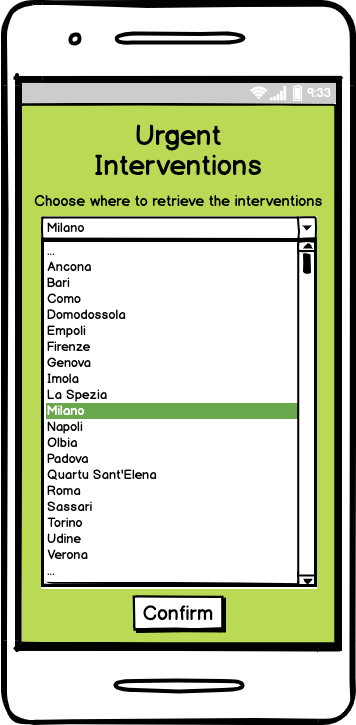
\includegraphics[width=0.6\textwidth]{/mockups/user/urgentInterventionsApp.png}
					\caption{\label{fig:urgentInterventionsApp} User Interventions}
				\end{minipage}\hfill
				\begin{minipage}{0.5\textwidth}
					\centering
					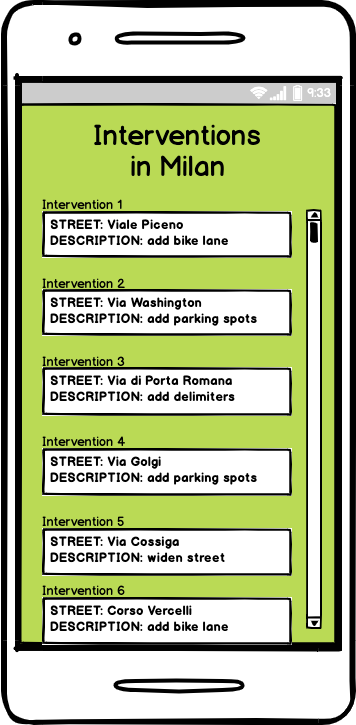
\includegraphics[width=0.6\textwidth]{/mockups/user/interventionsFoundApp.png}
					\caption{\label{fig:interventionsFoundApp} User Interventions Result}
				\end{minipage}
			\end{figure}
		
		\subsection[Authority Web App]{\hyperlink{toc}{Authority Web App}}
			\label{sec:authorityWebApp}
			
			Also in this case the layouts of the following mockups are only used to precisely describe how the functionalities of SafeStreets are provided to the authority. In this case we can consider the fact that the authorities do not necessarily need an interface that is very charming and pleasant while it is still very important to be intuitive. As in the mobile application, we have also here an interface that should be considered carefully in order to provide a clear description of the parking violations that have been reported to the authority (\autoref{sec:authorityUnreadReports}).
			
			\subsubsection[Login \& Registration]{\hyperlink{toc}{Login \& Registration}}
				\label{sec:authorityLoginRegistration}
				
				\paragraph{Login}
				The first mockup (\autoref{fig:loginWeb}) is the initial page each authority will find the first time he uses SafeStreets. Authorities can interact with the system only if authenticated. Hence the first time every authority will choose the button \textbf{sign up} for registering to the system and interact with the page described in the next paragraph.\\
				
				If an authority is already registered but has not chosen to be remembered, it will need to \textbf{login} to SafeStreets every time, by providing its PEC email and the password. Once recognized it will be redirected to the home page of the application described in the next section.\\
				
				This interface leads also to the possibility of recovering the credentials in case the authority forgets its password; also in this case, the mockup related to the link \textbf{Forgot Password} is not presented as it will simply ask the authority's email in order to send him its new password (it is supposed that authorities will never forget their PEC address).
				
				\vspace{0.6cm}
				
				\begin{figure}[ht!]
					\centering
					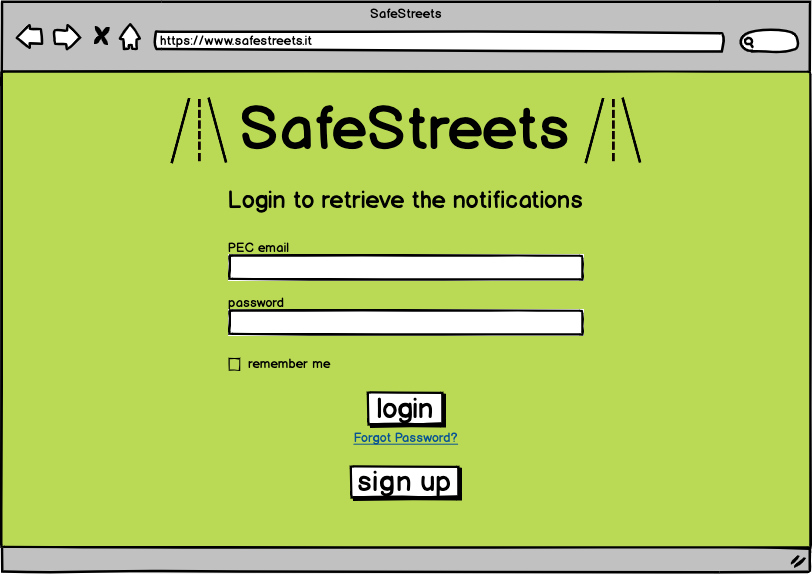
\includegraphics[scale=0.4]{/mockups/authority/loginWeb.png}
					\caption{\label{fig:loginWeb} Authority Login}
				\end{figure}
			
				\paragraph{Registration}
				The registration (\autoref{fig:registrationWeb}) allows the authority to create its account in order to be authenticated whenever it chooses to use SafeStreets. Thanks to this interface it will be able first to retrieve its city and provide the PEC email. Once the authority decides to send the verification code with the \textbf{send} button, the code will arrive to the PEC address of the authority that will insert it in the interface, choose the password and finally register. It is important to remember that also the authorities have to accept the \textbf{Terms and Conditions} of SafeStreets.\\
				
				The button \textbf{register} will add a new authority to the system and redirect to the login interface where the client can now access the system with the information provided in the previous module.
				
				\newpage
				
				\begin{figure}[ht!]
					\centering
					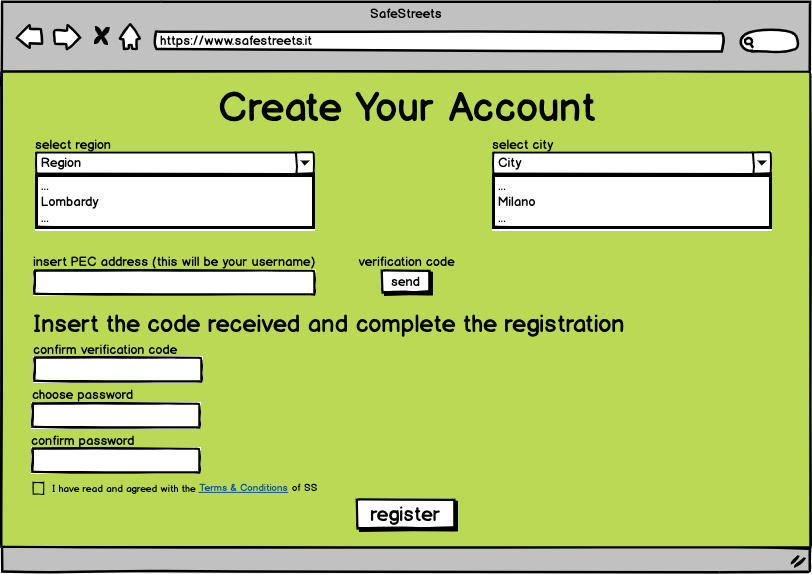
\includegraphics[scale=0.4]{/mockups/authority/registrationWeb.png}
					\caption{\label{fig:registrationWeb} Authority Registration}
				\end{figure}
			
			\subsubsection[Home Page]{\hyperlink{toc}{Home Page}}
				\label{sec:authorityHomePage}
				
				This page (\autoref{fig:homeWeb}) is the core of the interfaces, once logged the authority will reach it and after each action too. From the \textbf{Home Page} an authority is able to perform all the functionalities allowed to it, offered by SafeStreets:
				
				\begin{itemize}
					\item Check Unread Reports
					\item Find Reports
					\item Streets With Most Violations
					\item Find Dangerous Vehicles
					\item Find Unsafe Streets
					\item Find Urgent Interventions
				\end{itemize}
			
				The \textbf{logout} button is used to log out of the application and thus redirection will lead to the login page.
				
				\newpage
				
				\begin{figure}[ht!]
					\centering
					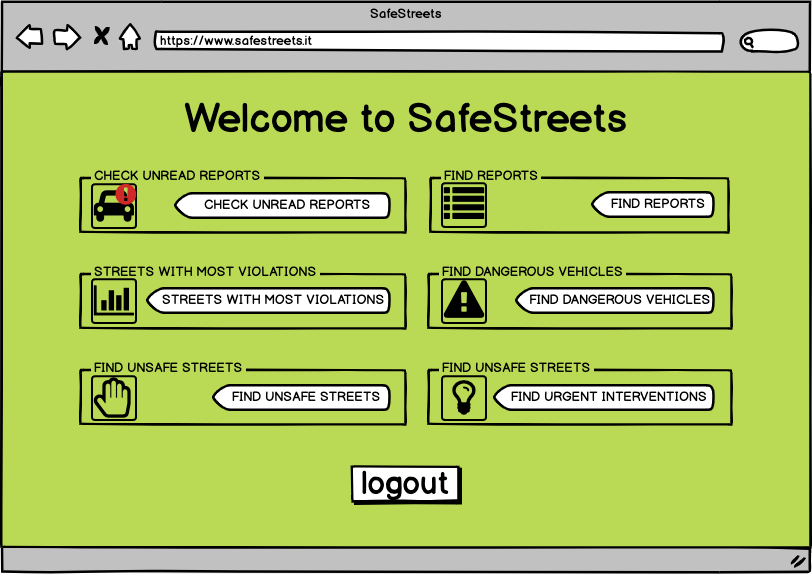
\includegraphics[scale=0.4]{/mockups/authority/homeWeb.png}
					\caption{\label{fig:homeWeb} Authority Home}
				\end{figure}
			
			\subsubsection[Unread Reports]{\hyperlink{toc}{Unread Reports}}
				\label{sec:authorityCheckReports}
				
				This page (\autoref{fig:unreadReports}) is the one that allows the notification of the authorities. As already described in the notification process, whenever a new report is accepted by the system it will be marked as unread for the authority that manages the relative street. This allows to notify the authority with all the reports that are not considered until the last check: if at least one report is present, the red exclamation icon will be displayed in the home page (\ref{sec:authorityHomePage}) and here a list of all the unread reports will be presented.\\
				
				Each report is described with the highest number of details possible: the ones provided by the users and those obtained by the system when validating the notification. \\
				
				Entering in this interface for the system means that the authority reads all the reports, hence after the redirection back to the home page, each notification will be marked as \textbf{read} and the red exclamation mark will not be present anymore: the list of unread reports is now empty.
				
				\newpage
				
				\begin{figure}[ht!]
					\centering
					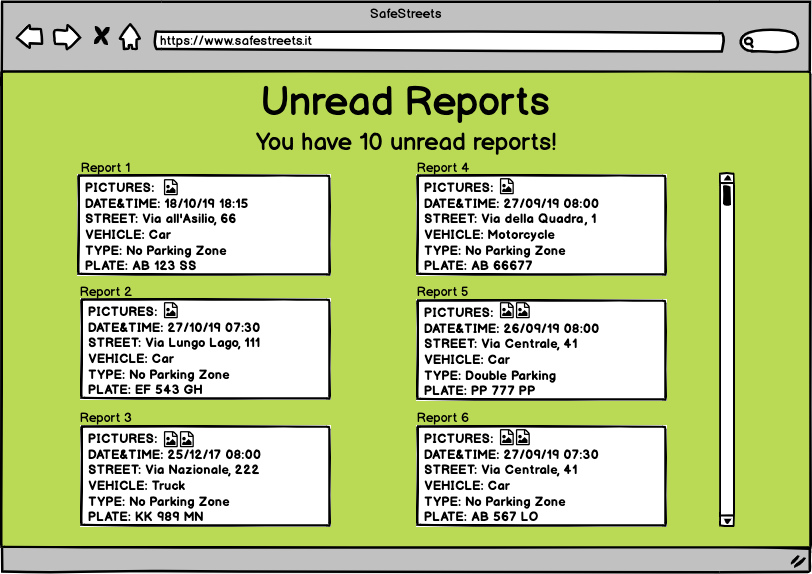
\includegraphics[scale=0.4]{/mockups/authority/unreadReportsWeb.png}
					\caption{\label{fig:unreadReports} Authority Notification}
				\end{figure}
			
			\subsubsection[Find Reports]{\hyperlink{toc}{Find Reports}}
				\label{sec:authorityFindReports}
				
				This interface (\autoref{fig:findReportsWeb}) is an authority only page that allows it to retrieve any kind of report stored in the system, related to its competent area (if a different city is selected, the system will not provide any result displaying an alert of selecting the correct city). This functionality in fact is given only to authorities in order to provide them a different level of visibility of the reports.\\
				
				Thanks to this interface the authority is able to retrieve all the reports that match the filters selected:
				
				\begin{itemize}
					\item \textbf{area:} by city and street
					\item \textbf{date:} periods of time are defined with an initial and a final date
					\item \textbf{time:} time slots of one hour each
					\item \textbf{type of violation:} different types of parking violations possible
					\item \textbf{type of vehicle:} different types of vehicle possible
				\end{itemize} 
			
				Once the authority has chosen the parameters and pressed the \textbf{Confirm} button, a list of all the reports that match the filters will be displayed as the result (\autoref{fig:reportsFoundWeb}). In this page the authority is able to see the details of each notification as they are stored in the system, hence with the highest level of visibility possible.\\
				
				\newpage
				
				\begin{figure}[ht!]
					\centering
					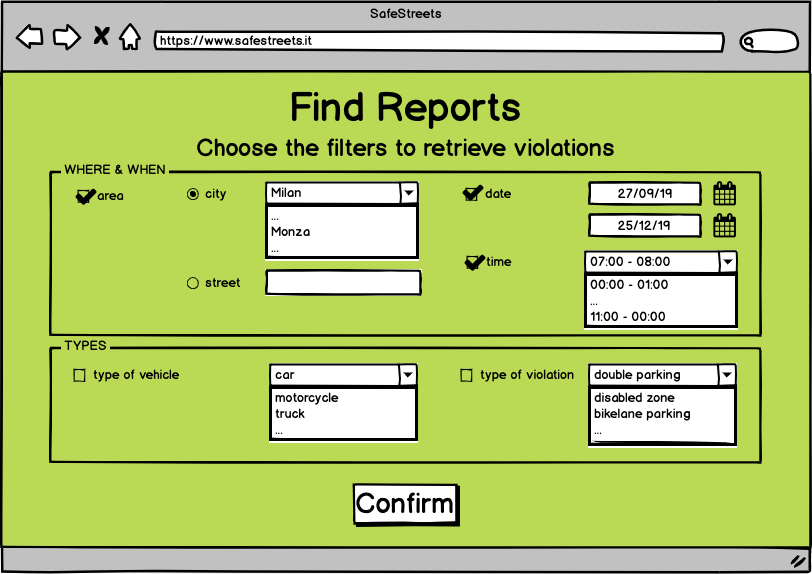
\includegraphics[scale=0.4]{/mockups/authority/findReportsWeb.png}
					\caption{\label{fig:findReportsWeb} Authority Find Reports}
				\end{figure}
			
				\vspace{1cm}
			
				\begin{figure}[ht!]
					\centering
					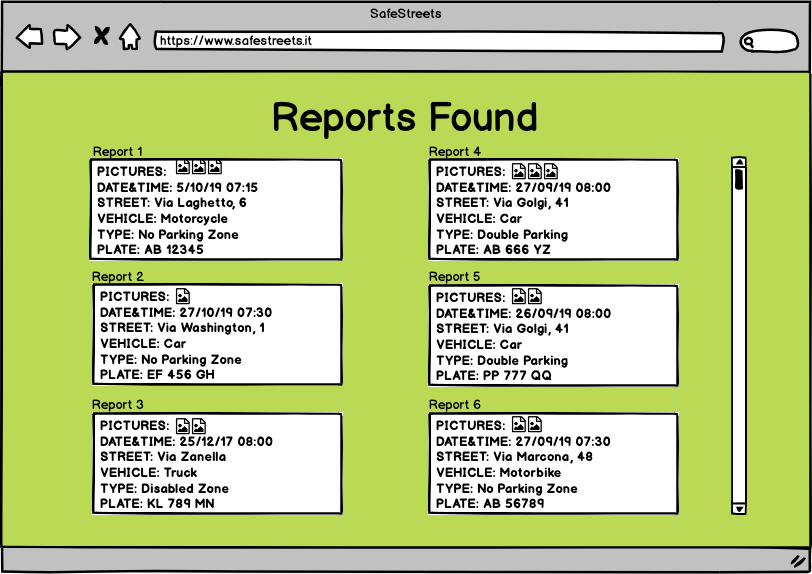
\includegraphics[scale=0.4]{/mockups/authority/reportsFoundWeb.png}
					\caption{\label{fig:reportsFoundWeb} Authority Reports Found}
				\end{figure}
			
				\newpage
			
			\subsubsection[Basic Functionalities]{\hyperlink{toc}{Basic Functionalities}}
				\label{sec:authorityBasicFunctionalities}
				
				These mockups are the ones that allow the authority to benefit of the basic functionalities, such as: mining the number of violations in a particular place or the vehicles that commit the most violations. The functionalities are the same of the users but presented in a web designed page: filters will be displayed for both pages, depending on the request that can be performed in that functionality.
				
				\paragraph{Streets With Most Violations}
				This page (\autoref{fig:violationsFrequencyWeb}) is used to mine the information about the frequency of the violations that have already occurred. Data can be retrieved with different levels of aggregation thanks to the possible filters:
				
				\begin{itemize}
					\item \textbf{area:} by city or everywhere
					\item \textbf{time:} time slots of one hour each
					\item \textbf{type of violation:} different types of parking violations possible
					\item \textbf{type of vehicle:} different types of vehicle possible
				\end{itemize}
			
				Selected the filters and the parameters for each filter chosen, the authority confirms the request with the \textbf{Confirm} button and receives the list of all the streets contained in the parking violations  that match the parameters, ordered by the number of infractions.\\
				
				The mockup related to the result of this functionality is not presented because it simply has to display the list of the streets found and allow the user to get back to the home page.
				
				\vspace{0.1cm}
				
				\begin{figure}[ht!]
					\centering
					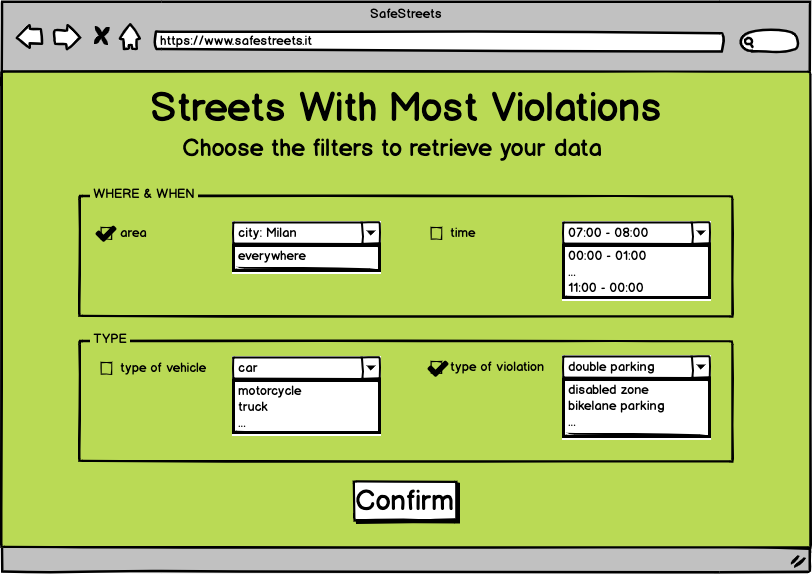
\includegraphics[scale=0.4]{/mockups/authority/violationsFrequencyWeb.png}
					\caption{\label{fig:violationsFrequencyWeb} Authority Violations Frequency}
				\end{figure}
				
				\paragraph{Dangerous Vehicles}
				This page (\autoref{fig:dangerousVehiclesWeb}) is used to mine the information about the vehicles that commit the highest number of parking violations. As well as in the first functionality we have filters to retrieve the data, but only the ones that are interesting for this kind of request:
				
				\begin{itemize}
					\item \textbf{area:} by city, street or everywhere
					\item \textbf{time:} time slots of one hour each
					\item \textbf{type of violation:} different types of parking violations possible
				\end{itemize}
			
				Selected the filters and the parameters for each filter chosen, the authority confirms the request with the \textbf{Confirm} button and receives the list of all the type of vehicles contained in the parking violations that match the parameters, ordered by the number of infractions.\\
				
				The mockup related to the result of this functionality is not presented because it simply has to display the list of the type of vehicles found and allow the user to get back to the home page.
				
				 \vspace{0.6cm}
				
				\begin{figure}[ht!]
					\centering
					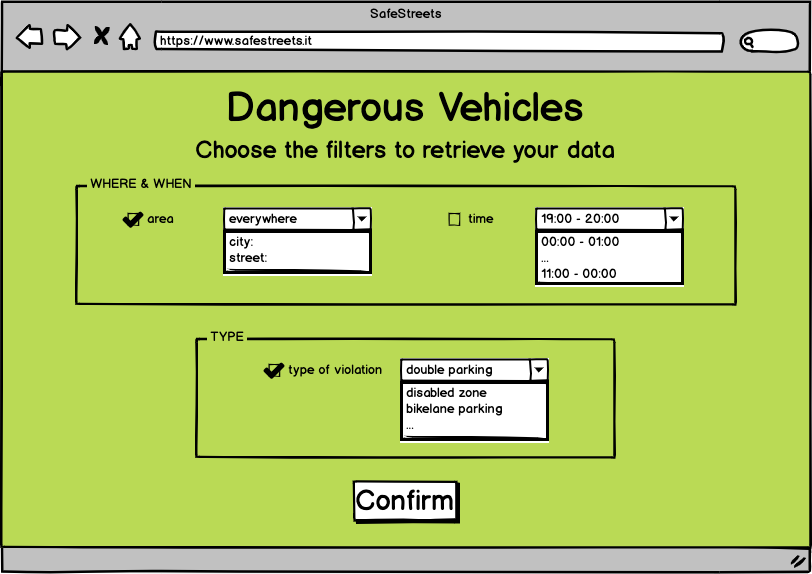
\includegraphics[scale=0.4]{/mockups/authority/dangerousVehiclesWeb.png}
					\caption{\label{fig:dangerousVehiclesWeb} Authority Dangerous Vehicles}
				\end{figure}
			
			\subsubsection[Advanced Functionalities]{\hyperlink{toc}{Advanced Functionalities}}
				\label{sec:authorityAdvancedFunctioalites}
				
				These mockups are the ones that allow the authority to benefit of the advanced functionalities, such as: finding the safety of the streets and receive a suggestion for a possible intervention that can be considered in order to enhance the safety of a dangerous street. Also in this case the functionalities are the same of the users' and thus we will have filters for the area of the unsafe streets and one only to choose the city where to retrieve the interventions.
				
				\paragraph{Unsafe Streets}
				This page (\autoref{fig:unsafeStreetsWeb}) is the only one that reflects the safety functionality, in face whenever the authority confirms the request with the \textbf{Confirm} button, the map on the bottom will be highlighted in green and red depending on the safety of the streets of interest. The selection of the area can be done in three different ways thanks to the filters provided by the interface:
				
				\begin{itemize}
					\item \textbf{city:} list of all the Italian cities
					\item \textbf{path:} two cells allow to select the starting (A) and the ending (B) point, the system will highlight the streets in the best path from A to B
					\item \textbf{street:} free choice of the user, a comma has to divide the street from the city
				\end{itemize}
				
				Once the authority has chosen the area to highlight the safety and pressed the \textbf{Confirm} button, the map will be updated following on either the street or the path or the city; in this last case a high view of the city will be displayed and the authority will be able to zoom in and out to select the places it prefers.
				
				\vspace{0.6cm}
					
				\begin{figure}[ht!]
					\centering
					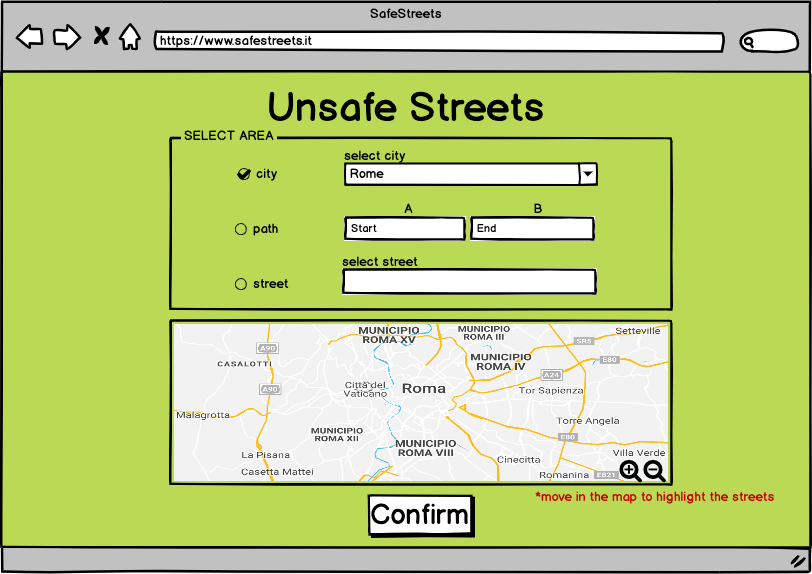
\includegraphics[scale=0.4]{/mockups/authority/unsafeStreetsWeb.png}
					\caption{\label{fig:unsafeStreetsWeb} Authority Unsafe Streets}
				\end{figure}
			
				\paragraph{Urgent Interventions}
				This page (\autoref{fig:urgentInterventionsWeb}) allows the authority to retrieve the suggestions for the possible interventions in the city it selects. The \textbf{Confirm} button will lead to the result providing a list of all the interventions found in that city.\\
				
				In this case we provide also the page of the results (\autoref{fig:unsafeStreetsWeb}) as it is important to show which kind of information this request will display. As we see in the result, for each intervention is is provided the street and the suggestion, in case a street has multiple suggestions, two interventions in the same street but with different suggestion will be presented.
				
				\vspace{0.4cm}				
				
				\begin{figure}[ht!]
					\centering
					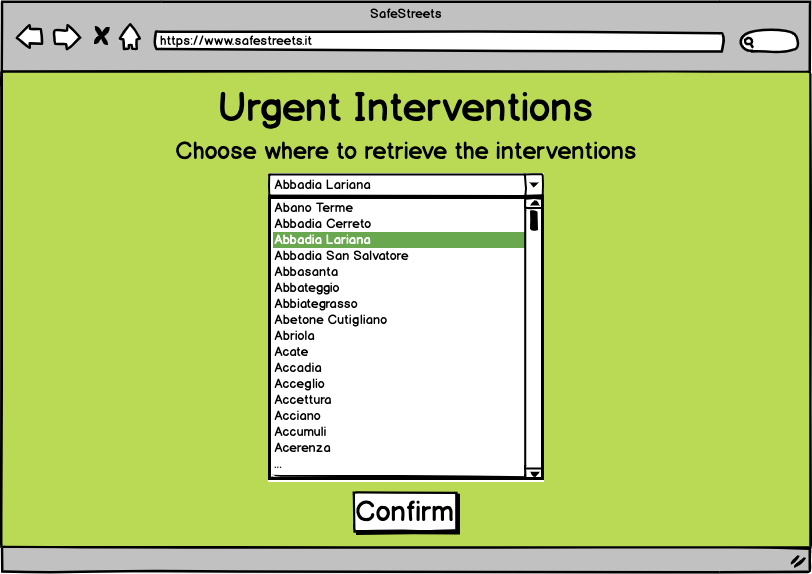
\includegraphics[scale=0.4]{/mockups/authority/urgentInterventionsWeb.png}
					\caption{\label{fig:urgentInterventionsWeb} Authority Interventions}
				\end{figure}
			
				\begin{figure}[ht!]
					\centering
					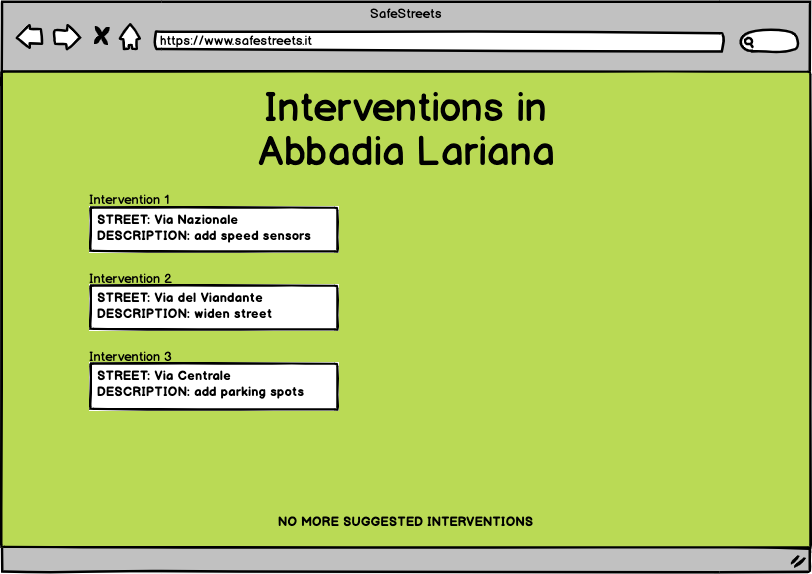
\includegraphics[scale=0.4]{/mockups/authority/interventionsFoundWeb.png}
					\caption{\label{fig:interventionsFoundWeb} Authority Interventions Result}
				\end{figure}